\chapter{Introduction}
\label{ch:intro}
\pagenumbering{arabic}

The increasing popularity and the intensive use of computational systems in the everyday of modern life create the need for easier and less invasive forms of user recognition. While enter a hard to memorize password in a terminal and identify a person placing a human to listen to telephone calls are the status quo for respectively authentication and identification, voice biometrics presents itself as a continuing improvement alternative. Passwords can be forgotten and people are biased and unable to be massive trained, but the unique characteristics of a person's voice combined with an Automatic Speaker Recognition (ASR) system outperform any ``manual" attempt.

Speech is the most natural way humans have to communicate, being incredibly complex and with numerous specific details related to its producer, \refbib{Bimbot et al.}{bimbot.et.al.2004}. Therefore, it is expected an increasing use of vocal interfaces to perform actions such as computer login, voice search (e.g., Apple Siri, Google Now and Samsung S Voice) and identification of speakers in a conversation and its content. Nowadays, fingerprint biometrics is present in several solutions (e.g., ATMs, \refbib{Wang \& Wu}{wang.wu.2002}), authentication through facial recognition comes as built-in software for average computers and iris scan was adopted for a short time by United Kingdom's and permanently by United Arab Emirates' border controls, \refbib{Sasse}{sasse.2007}, \refbib{Raisi \& Khouri}{raisi.khouri.2008}. These examples indicate a near future where biometrics are common, with people talking to the computer and receiving concise answers, and cash withdrawals allowed via a combination of speaker verification, correctly dictated captcha and any other technique.

Current commercial products based on voice technology (e.g., Dragon Naturally Speaking, KIVOX and VeriSpeak) are usually intended to perform either \textbf{speech recognition} (\emph{what} is being said) or \textbf{speaker recognition} (\emph{who} is speaking). Voice search applications are designed to determine the content of a speech, usually with no concern about who the speaker is or if there is more than one, while computer login and telephone fraud prevention supplement a memorized personal identification code with speaker verification, \refbib{Reynolds}{reynolds.1995a}, not interested on the message spoken. Few applications perform both processes, such as automatic speaker labeling of recorded meetings, that transcribes what each person is saying. To achieve these goals, numerous voice processing techniques have become known in academy and industry, such as Natural Language Processing (NLP), Hidden Markov Models (HMMs) and Gaussian Mixture Models (GMMs). Although all of these are interesting state-of-the-art techniques, this paper covers a subarea of speaker recognition and only a small subset will be unraveled.

\section{Speaker Recognition}
\label{sec:speaker-recognition}

As stated in \refbib{Reynolds \& Campbell}{reynolds.campbell.2008}, speaker recognition may be divided in two subareas. The first is \textbf{speaker identification}, aimed to determine the identity of a speaker from a non-unitary set of known speakers. This task is also named speaker identification in \textbf{closed set}. In the second, \textbf{speaker verification}, the goal is to determine if a speaker is who he or she claims to be, not an imposter. As the set of imposters is unknown, this is an \textbf{open set} problem. An intermediate task is \textbf{open set identification}, when an ``unmatched class" is added in order to categorize all unknown speakers.

\begin{figure}[ht]
    \centering
    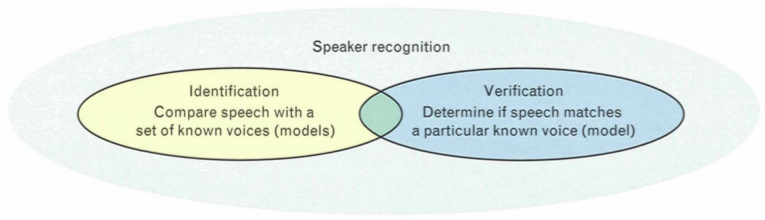
\includegraphics[width=\textwidth]{speaker-recognition}
    \caption{Relation between identification and verification of speakers, \refbib{Reynolds}{reynolds.1995a}.}
    \label{fig:speaker-recognition}
\end{figure}

The text inputted may have constraints, such as type (e.g., digits and letters), number of words used (e.g., one word or sentences) and etc. In \textbf{text-dependent} systems the content of the speech is relevant to the evaluation, and the testing texts must belong to the training set, \refbib{Hébert}{hebert.2008}. A change in the training inputs demands a complete new training section. \textbf{Text-independent} systems have no restrictions to the message in both sets, with the non-textual characteristics of the user's voice (e.g., pitch and accent) being the important aspects to the evaluator. These characteristics are present in different sentences, use of foreign languages and even gibberish. Between the extremes in constraints falls the \textbf{vocabulary-dependent system}, which restricts the speech to come from a limited vocabulary (e.g., digits such as ``two" or ``one-two-three"), \refbib{Reynolds}{reynolds.1995a}.

\section{Gaussian Mixture Models}
\label{sec:gmm}

The focus of this paper is on \textbf{text-independent speaker recognition} (both identification and verification), and as independence of the spoken context is a key characteristic of the problem, the most appropriate approach is to consider the training data as a stochastic variable. The best suited distribution to represent random data is the gaussian (or normal), leading to the choice of GMMs to model an ASR system.

Recognition systems are constructed using several techniques based on GMM. For the identification process a GMM is trained for each enrolled speaker, referred to as Gaussian Mixture Speaker Model (GMSM), with the identity given by the model with higher likelihood. Verification systems are designed using an Universal Background Model-Gaussian Mixture Model (UBM-GMM) trained to represent all speakers as a single background and a GMSM or a bayesian adaptation of the UBM-GMM, \refbib{Brown, Lee and Spohrer}{brown.lee.spohrer.1983}, named Adapted Gaussian Mixture Speaker Model (AGMSM). A likelihood ratio test is used to evaluate a speech signal and to decide if it belongs or not to the claimed speaker. All techniques are detailed in \chapterref{gmm}.

% possible paragraph about FCM + GMM

\section{Objectives}

This study is aimed to implement ASR systems (for both identification and verification processes) and analyze the following:

\begin{itemize}\itemsep0pt
    \item Correct identification rates for different sizes of mixture and features.
    \item False detection and false rejection rates for speaker verification using a DET curve, \refbib{Martin et al.}{martin.et.al.1997}.
    \item Accuracy of a speaker verification system for different sizes of mixture and features.
    \item Comparison between GMSM and AGMSM verifications.
    %\item [possible item] Improvement when using FCM
\end{itemize}

\section{Document Structure}

\chapterref{speaker-recognition-systems} contains basic information about ASR systems, as well as its basic architectures. The feature extraction process is explained in \chapterref{feature-extraction}, from the reasons for its use to the chosen technique (Mel-Frequency Cepstral Coefficient, MFCC). In \chapterref{gmm} the theories of GMM, UBM-GMM and AGMSM are presented. Experiments are described in \chapterref{experiments}, as well as its results. Finally, \chapterref{conclusion} concludes the study. Furthermore, important contents are presented in the appendices. \appendixref{gmsm-verify-results} shows the results and curves for GMSM verification and \appendixref{agmsm-verify-results} for AGMSM verification.